%% 2019 NeuroFedora contributors

%% packages %%
% support for coloured text
\usepackage{xcolor}
\definecolor{FedoraBlue}{cmyk}{1.0,0.46,0.0,0.0}
\definecolor{FedoraDarkBlue}{cmyk}{1.0,0.57,0.0,0.38}
\definecolor{FriendsMagenta}{cmyk}{0.0,0.8,0.4,0.0}
\definecolor{FeaturesOrange}{cmyk}{0.0,0.5,1.0,0.0}
\definecolor{FirstGreen}{cmyk}{0.5,0.0,1.0,0.0}
\definecolor{FreedomPurple}{cmyk}{0.57,0.46,0.0,0.0}

% IPA
\usepackage{tipa}
\usepackage[scale=2]{ccicons}
\usepackage{amssymb}
\usepackage{tikz}
\usetikzlibrary{arrows.meta, arrows, positioning}
\usepackage{jneurosci}
\usepackage{subfig}
\usepackage[T1]{fontenc}
\usepackage[utf8]{inputenc}
\usepackage[style=verbose,backend=biber,autocite=footnote]{biblatex}
\addbibresource{masterbib.bib}
% Use opensans
\usepackage[default,osfigures,scale=0.95]{opensans}
% for strike through
\usepackage[normalem]{ulem}
% links, urls, refs
\usepackage{hyperref}
\hypersetup{colorlinks,linkcolor=FreedomPurple,urlcolor=FreedomPurple}
% graphics
\usepackage{graphicx}
% algorithm
\usepackage{algorithmic}
\usepackage{textcomp}
\usepackage{wrapfig}
\usepackage{textgreek}
\usepackage{euler}
% \usepackage{minted}

% beamer theme
\usetheme[numbering=fraction]{metropolis}
\usefonttheme[onlymath]{serif}
\setbeamerfont{footnote}{size=\tiny}
\setbeamerfont{caption}{size=\tiny}
\setbeamercolor{alerted text}{fg=FeaturesOrange}
\setbeamercolor{progress bar}{fg=FriendsMagenta}
\setbeamercolor{title separator}{fg=FriendsMagenta}
\setbeamercolor{frametitle}{bg=FedoraDarkBlue}

\renewcommand{\figurename}{}

% Not needed in metropolis, but in general footnote citation fixes: https://tex.stackexchange.com/questions/44217/how-can-i-stop-footcite-from-hijacking-my-beamer-columns
% how to use multiple references to the same footnote: https://tex.stackexchange.com/questions/27763/beamer-multiple-references-to-the-same-footnote

%% title %%
\title[NeuroFedora]{
\includegraphics[keepaspectratio,width=.25\textwidth]{images/NeuroFedoraLogo01.png}\\NeuroFedora}
\subtitle{Free Software for Free Neuroscience}
\author{NeuroFedora Contributors}
%\author{Ankur Sinha\\Ph.D. candidate: UH Biocomputation Group, UK,\\Volunteer: Fedora Project.}
\date[]{}
%% document begins %%
\begin{document}

% title frame %%
\begin{frame}
  \titlepage{}
\end{frame}

%% Three slides for 5 minutes, so 9 slides for 15 minutes.
\section{How: Research Pipeline}

\begin{frame}[c]{General workflow}
	\begin{figure}[h]
		\centering
%		\only<1>{\tikzset{
    %Define standard arrow tip
    >=stealth',
    %Define style for boxes
    punkt/.style={
           circle,
           draw=black, very thick,
           text=FedoraDarkBlue,
           text width=6em,
           minimum height=2em,
           text centered},
    % Define arrow style
    pil/.style={
           <-,
           very thick,
           draw=FreedomPurple,
           shorten <=2pt,
           shorten >=2pt,}
}
\begin{tikzpicture}[node distance=1cm, auto,]
 %nodes
 \node[punkt, draw=FedoraBlue, text=FedoraBlue] (experiments) {Experimental work};
 \node[punkt, draw=FriendsMagenta, text=FriendsMagenta, above right=of experiments]
 (analysis) {Data analysis}
 edge[pil, bend right=45] (experiments.north);
 \node[punkt, draw=FeaturesOrange, text=FeaturesOrange, below right=of analysis]
 (theory) {Theory}
 edge[pil, bend right=45] (analysis.east);
 \node[punkt, draw=FirstGreen, text=FirstGreen, below left=of theory]
 (modelling) {Modelling}
 edge[pil, bend right=45] (theory.south)
 edge[pil, ->, bend left=45] (experiments.south);
 % We make a dummy figure to make everything look nice.
 % \node[above=of market] (dummy) {};
 % \node[right=of dummy] (t) {Ultimate borrower}
   % edge[pil,bend left=45] (market.east) % edges are used to connect two nodes
   % edge[pil, bend left=45] (formidler.east); % .east since we want
                                             % % consistent style
 % \node[left=of dummy] (g) {Ultimate lender}
   % edge[pil, bend right=45] (market.west)
   % edge[pil, bend right=45] (formidler.west)
   % edge[pil,<->, bend left=45] node[auto] {Direct (a)} (t);
\end{tikzpicture}
}%
		\only<1>{\tikzset{
    %Define standard arrow tip
    >=stealth',
    %Define style for boxes
    punkt/.style={
           circle,
           draw=black, very thick,
           text=FedoraDarkBlue,
           text width=6em,
           minimum height=2em,
           text centered},
    % Define arrow style
    pil/.style={
           <-,
           very thick,
           draw=FreedomPurple,
           shorten <=2pt,
           shorten >=2pt,}
}
\begin{tikzpicture}[node distance=1cm, auto,]
 %nodes
 \node[punkt, draw=FedoraBlue, text=FedoraBlue] (experiments) {Experimental work};
 \node[punkt, draw=FriendsMagenta, text=FriendsMagenta, above right=of experiments]
 (analysis) {Data analysis}
 edge[pil, ->, bend left=45, opacity=0.4] (experiments.east)
 edge[pil, bend right=45] (experiments.north);
 \node[punkt, draw=FeaturesOrange, text=FeaturesOrange, below right=of analysis]
 (theory) {Theory}
 edge[pil, bend right=45] (analysis.east)
 edge[pil, ->, bend left=45, opacity=0.4] (analysis.south);
 \node[punkt, draw=FirstGreen, text=FirstGreen, below left=of theory]
 (modelling) {Modelling}
 edge[pil, bend right=45] (theory.south)
 edge[pil, ->, bend left=45] (experiments.south)
 edge[pil, ->, bend left=45, opacity=0.4] (theory.west)
 edge[pil, <-, bend right=45, opacity=0.4] (experiments.east)
 edge[pil, ->, bend left=45, opacity=0.4] (analysis.south)
 edge[pil, <-, bend right=45, opacity=0.4] (analysis.south);
 % We make a dummy figure to make everything look nice.
 % \node[above=of market] (dummy) {};
 % \node[right=of dummy] (t) {Ultimate borrower}
   % edge[pil,bend left=45] (market.east) % edges are used to connect two nodes
   % edge[pil, bend left=45] (formidler.east); % .east since we want
                                             % % consistent style
 % \node[left=of dummy] (g) {Ultimate lender}
   % edge[pil, bend right=45] (market.west)
   % edge[pil, bend right=45] (formidler.west)
   % edge[pil,<->, bend left=45] node[auto] {Direct (a)} (t);
\end{tikzpicture}
}
		\note[item]{A simplified diagram. Actually a lot more complex}
		\note[item]{General workflow of research-based work.}
		\note[item]{Most work now-a-days is being carried out with the use of computer software, such as ...}
	\end{figure}
\end{frame}

\begin{frame}[c]{Tools of the trade}
	\textcolor{FedoraBlue}{Experimental:}
	\begin{itemize}
		\item EEG, ECoG, intracellular and extracellular single and multi neuron recording,
		\item CT, DOI, MRI, f-MRI, MEG, PET,
	\end{itemize}
	\textcolor{FriendsMagenta}{Data analysis:}
	\begin{itemize}
		\item Statistics,
		\item Machine Learning, Big Data, Deep learning,
	\end{itemize}
	\textcolor{FeaturesOrange}{Theory} and \textcolor{FirstGreen}{modelling:}
	\begin{itemize}
		\item Simulators of all kinds, 
	\end{itemize}
	\note[item]{Experimental: DICOM/Image viewers, fsl tools, software to drive the big machines}
	\note[item]{Data Analysis: Simple/complex libraries, from numpy, scipy to scikit-learn, tensorflow}
	\note[item]{Simulators: Neuron, NEST, plenty more...}
	\note[item]{Lots of hardware and software is required for basic neuroscience research.}
\end{frame}

\begin{frame}[c]{Tools of the trade:\ II}
	\textcolor{FedoraDarkBlue}{Tools for the dissemination of knowledge\footnotemark[4]:}
	\begin{itemize}
		\item visualisation,
		\item academic writing,
		\item non academic writing: blogging \ldots,
		\item pod-casting,
		\item video making,
		\item creating teaching materials,
		\item collaborative tools and utilities
	\end{itemize}
	\footnotetext[4]{also to a non-specialist audience.}
	\note[item]{common tools used by people in science and research}
\end{frame}

\section{Free/Open (neuro) Science}
\begin{frame}[c]{The ideal, in short:}
	Free/Open Science:\\\alert{Everyone} should have the freedom to \alert{share, study, and modify} scientific material.\\
	
	\vspace{0.5cm}
	FOSS\@:\\\alert{Everyone} should have the freedom to \alert{share, study, and modify} software\footnotemark[5].\\
	\footnotetext[2]{\href{https://u.fsf.org/user-liberation}{Free software foundation}}
	
	\vspace{0.5cm}
	\alert{Free/Open Science includes and relies heavily on Free/Open Source Software (FOSS).}
	\note[item]{simple definitions}
\end{frame}

\begin{frame}[c]{So we strive to use more and more FOSS}
	\begin{figure}[htpb]
		\centering
		
\includegraphics[width=\linewidth]{images/open-source-paper.png}
	\end{figure}
	\footnotetext[6]{\href{http://opensourceforneuroscience.org/}{Open source for neuroscience}}
	\note[item]{reproducibility crisis. unable to reproduce data, results}
	\note[item]{benefits of open-sourcing code. helps community. reuse. build-on and improve. publication becomes an advert for the code.}
\end{frame}

\section{NeuroFedora: why, how, what?}

\begin{frame}[c]{Neuroscience community: highly multidisciplinary}
	\begin{itemize}
		\item \alert{various specialities:} biologists, mathematicians, physicists, chemists, psychologists, \ldots, 
		\item \alert{small proportion of trained software developers}
	\end{itemize}
	\note[item]{Full of people from various fields}
	\note[item]{Not all have the required XP}
\end{frame}

\begin{frame}[c]{FOSS:\ Developers and users}
	\begin{figure}[h]
		\begin{center}
			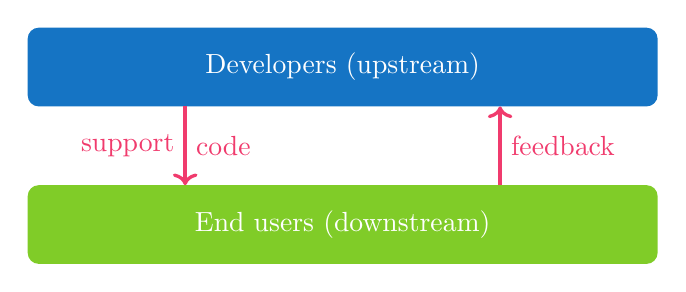
\begin{tikzpicture}[scale=1, transform shape]
			\fill[fill=FedoraBlue, text=white, rounded corners] (0, 0) rectangle ++(8, 1) node[pos=0.5] (A){Developers (upstream)};
			\fill[fill=FirstGreen, text=white, rounded corners] (0, -2) rectangle ++(8, 1) node[pos=0.5] (B){End users (downstream)};
			\draw [FriendsMagenta, very thick, ->] (2, 0) -- node [midway, right, text centered] {code} node [midway, left, text centered] {support} ++(0, -1) ;
			\draw [FriendsMagenta, very thick, ->] (6, -1) -- node [midway, right, text centered] {feedback} ++(0, 1);
			\end{tikzpicture}
		\end{center}
	\end{figure}
	\note[item]{The dev may not provide instructions on how to use the software}
	\note[item]{Difficult for people who lack programming knowledge to build/use the tool directly from the dev.}
	\note[item]{End users not always provide feedback}
\end{frame}

\begin{frame}[c]{(Anecdotal) notes on development of research software}
	\begin{itemize}
		\item often \alert{single developer}, or small development teams
		\item limited \alert{maintenance, short-lived projects}
		\item limited \alert{access to hardware/resources}
		\item limited \alert{code quality}
		\item limited \alert{use of established best practices}
		\item limited \alert{testing for correctness (!)}
		\item \alert{complex dependency chains}
		\item lack of \alert{documentation and support}
		\item lack of \alert{community development know-how}
	\end{itemize}
	\note[item]{Given how interdisciplinary neuroscience is, most researchers are NOT trained in development}
	\note[item]{based on anecdotal evidence, software used in research is not of the best quality}
	\note[item]{may or may neet development standards}
	\note[item]{may have an instruction set on how to install/use the software}
	\note[item]{resolving dependencies can be difficult}
\end{frame}

\begin{frame}[c]{(Anecdotal) notes on users of research software}
	\begin{itemize}
		\item \alert{waste time and effort} installing (and reinstalling) their software stacks
		\item \alert{rarely run test suites (!)}
		\item \alert{rarely report bugs} upstream
		\item \alert{rarely send improvements} upstream
		\item are \alert{unaware of helpful development tools}
	\end{itemize}
	\note[item]{The other side of the bridge is the users}
	\note[item]{also suffer from resolving dependencies}
	\note[item]{lack the required skill/knowledge of programming, they have a hard time setting up and using the software}
	\note[item]{If correctness of a tool cannot be verified, how can the correctness of the scientific result be claimed?}
\end{frame}

\begin{frame}[c]{Distributions liaison between developers and users}
	\begin{figure}[h]
		\begin{center}
			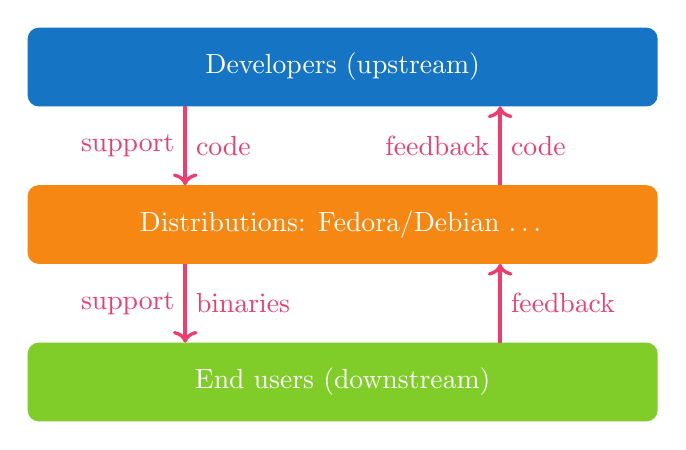
\begin{tikzpicture}[scale=1, transform shape]
			\fill[fill=FedoraBlue, text=white, rounded corners] (0, 0) rectangle ++(8, 1) node[pos=0.5] (A){Developers (upstream)};
			\fill[fill=FeaturesOrange, text=white, rounded corners] (0, -2) rectangle ++(8, 1) node[pos=0.5] (B){Distributions: Fedora/Debian \ldots};
			\draw [FriendsMagenta, very thick, ->] (2, 0) -- node [midway, right, text centered] {code} node [midway, left, text centered] {support} ++(0, -1) ;
			\draw [FriendsMagenta, very thick, ->] (6, -1) -- node [midway, right, text centered] {code} node [midway, left, text centered] {feedback} ++(0, 1) ;
			\fill[fill=FirstGreen, text=white, rounded corners] (0, -4) rectangle ++(8, 1) node[pos=0.5] (B){End users (downstream)};
			\draw [FriendsMagenta, very thick, ->] (2, -2) -- node [midway, right, text centered] {binaries} node [midway, left, text centered] {support} ++(0, -1) ;
			\draw [FriendsMagenta, very thick, ->] (6, -3) -- node [midway, right, text centered] {feedback} ++(0, 1) ;
			\end{tikzpicture}
		\end{center}
	\end{figure}
	\note[item]{role of distros:}
	\note[item]{liaison between the users and developers}
	\note[item]{provide feedback, report bugs to the dev}
	\note[item]{simplify installation/usage XP}
\end{frame}

\begin{frame}[c]{Distributions, like Fedora, are in a unique position:}
	\begin{itemize}
		\item \alert{liaison between upstream and users}
		\item have the \alert{infrastructure}
		\item \alert{follow best practices} in software development
		\item constantly \alert{work on community development}
		\item \alert{learn from one another}---train while working
		\item \alert{disseminate} information to end-users
	\end{itemize}
	\note[item]{high end servers. multiple mirrors across the globe}
	\note[item]{firm packaging guidelines; go through a heavy-duty review process; proper testing of the software before releasing to the general user}
	\note[item]{many contributors hail from different backgrounds, and have a lot to learn}
	\note[item]{provide help to the users}
\end{frame}

\begin{frame}[c]{NeuroFedora:}
	\textcolor{FedoraBlue}{Primary goal:}
	\begin{itemize}
		\item Provide a \alert{ready to use, integrated FOSS platform} for neuroscientists\footnotemark[7].
	\end{itemize}
	\textcolor{FirstGreen}{Secondary/collateral goals:}
	\begin{itemize}
		\item help \alert{improve the standard and maintenance} of tools
		\item help users \alert{develop software development skills}
		\item \alert{make neuroscience accessible} to non-specialists
	\end{itemize}
	\footnotetext[7]{Researchers, academics, hobbyists, anyone!}
\end{frame}

\begin{frame}[c]{NeuroFedora: current metrics}
	\begin{itemize}
		\item \alert{Turned a year old, in September 2019\footnotemark[8],}
		\item \textcolor{FirstGreen}{20 volunteers}
		\begin{itemize}
			\item 16 package maintainers
			\item 5 designers, newcomers
			\item only 5 from a neuroscience background
		\end{itemize}
		\item \textcolor{FriendsMagenta}{software:}
		\begin{itemize}
			\item 135 tools (packages) ready to install\footnotemark[9]:
			\begin{itemize}
				\item Neuron, InterViews, NEST, Genesis, Brian (v1 and v2), Moose, python-libNeuroML, PyLEMS, PyNWB, \ldots
			\end{itemize}
			\item \textasciitilde{}180 in queue\footnotemark[10].
			\begin{itemize}
				\item NeuroMLlite, pyNeuroML, NetPyNE, \ldots
			\end{itemize}
		\end{itemize}
	\end{itemize}
	% hardcoding some spaces, just to make them look neat.
	\footnotetext[8]{\ \ \ in its second iteration}
	\footnotetext[9]{\href{https://src.fedoraproject.org/group/neuro-sig}{\ \ \ src.fedoraproject.org: Neuro-SIG}}
	\footnotetext[10]{\href{https://pagure.io/neuro-sig/NeuroFedora/issues?status=Open&tags=T\%3A+Software}{\ \ \ Pagure.io: Neuro-SIG: issues}}
\end{frame}

\begin{frame}[c]{Search: ``NeuroFedora''}
	\begin{columns}
		\begin{column}{0.3\textwidth}
			\begin{figure}[h]
				\centering
				
\includegraphics[width=\linewidth]{images/NeuroFedoraBadge.png}
			\end{figure}
		\end{column}
		\begin{column}{0.8\textwidth}
			\textcolor{FedoraBlue}{Mailing list:\ neuro-sig@lists.fedoraproject.org}\\
			\textcolor{FirstGreen}{IRC:\ \#fedora-neuro on Freenode}\\
			\textcolor{FeaturesOrange}{Telegram:\ t.me/NeuroFedora}\\
			\textcolor{FriendsMagenta}{Documentation\ neuro.fedoraproject.org}\\
			\textcolor{FirstGreen}{Blog:\ neuroblog.fedoraproject.org}\\
			\textcolor{FeaturesOrange}{Pagure.io (FOSS Git forge):\ neuro-sig/NeuroFedora}
		\end{column}
	\end{columns}
\end{frame}

\end{document}
